\documentclass{article}

\usepackage[margin=1in]{geometry}
\usepackage{amsmath}
\usepackage{graphicx}
\usepackage{float}
\usepackage[hidelinks]{hyperref}

\graphicspath{{llm_similarity/round6/relative_output/}}

\title{Two-Stage Relative Similarity Exercise}
\author{}
\date{}

\begin{document}
\maketitle

\section{Method}

The exercise considers the Control, Market, Aid, and Bonus versions of DG-KW,
UG, and TG. For Aid and Bonus, the story precedes the corresponding game
instructions, as in the experiment. Contexts and vignettes are presented under
neutral identifiers, without their game or representation labels.

Three separate Codex agents independently complete every rating task. Each
agent reads the target game--frame context and all vignettes in the specified
choice set, then allocates exactly 1,000 integer points across them. More
points indicate greater similarity. Thus, if $p_{acv}$ denotes the points
allocated by agent $a$ to vignette $v$ for context $c$,

\begin{equation}
    p_{acv}\geq 0, \qquad \sum_{v\in\mathcal{V}_{c}}p_{acv}=1{,}000.
\end{equation}

This is a direct relative judgment: it is not constructed by normalizing the
earlier independent 0--100 similarity scores. The exercise proceeds in two
stages, separating similarity in game structure from similarity among
representations within a fixed game structure. Each agent receives a
separately shuffled packet containing only neutral identifiers and texts.
The agents were instructed to use only their packet and not to access the
classification map, one another's packets or ratings, the earlier ratings,
or the resulting figures. We average the three point allocations vignette by
vignette before aggregation. These are independent rating passes from
separate agents, although they are not a test of robustness across different
model families.

\section{Stage 1: similarity to vignette game structures}

In the first stage, each of the 12 game--frame contexts is compared jointly
with all 30 vignettes. The vignettes comprise 6 DG, 12 UG, and 12 TG cases.
Because these families contain different numbers of vignettes, the comparison
uses the mean allocated points per vignette in family $g$ after averaging
across the three agents,

\begin{equation}
    \bar p_{cv}=\frac{1}{3}\sum_{a=1}^{3}p_{acv},
    \qquad
    \mu_{cg}=\frac{1}{|\mathcal{V}_{g}|}
    \sum_{v\in\mathcal{V}_{g}}\bar p_{cv},
    \qquad
    s_{cg}=\frac{\mu_{cg}}{\sum_h\mu_{ch}}.
\end{equation}

Using family totals instead would mechanically favor the two families with
twice as many vignettes. We therefore normalize the three family means so that
$\sum_g s_{cg}=1$ within each target context. Figure~\ref{fig:structural-control}
reports these normalized shares in Control.

\begin{figure}[H]
    \centering
    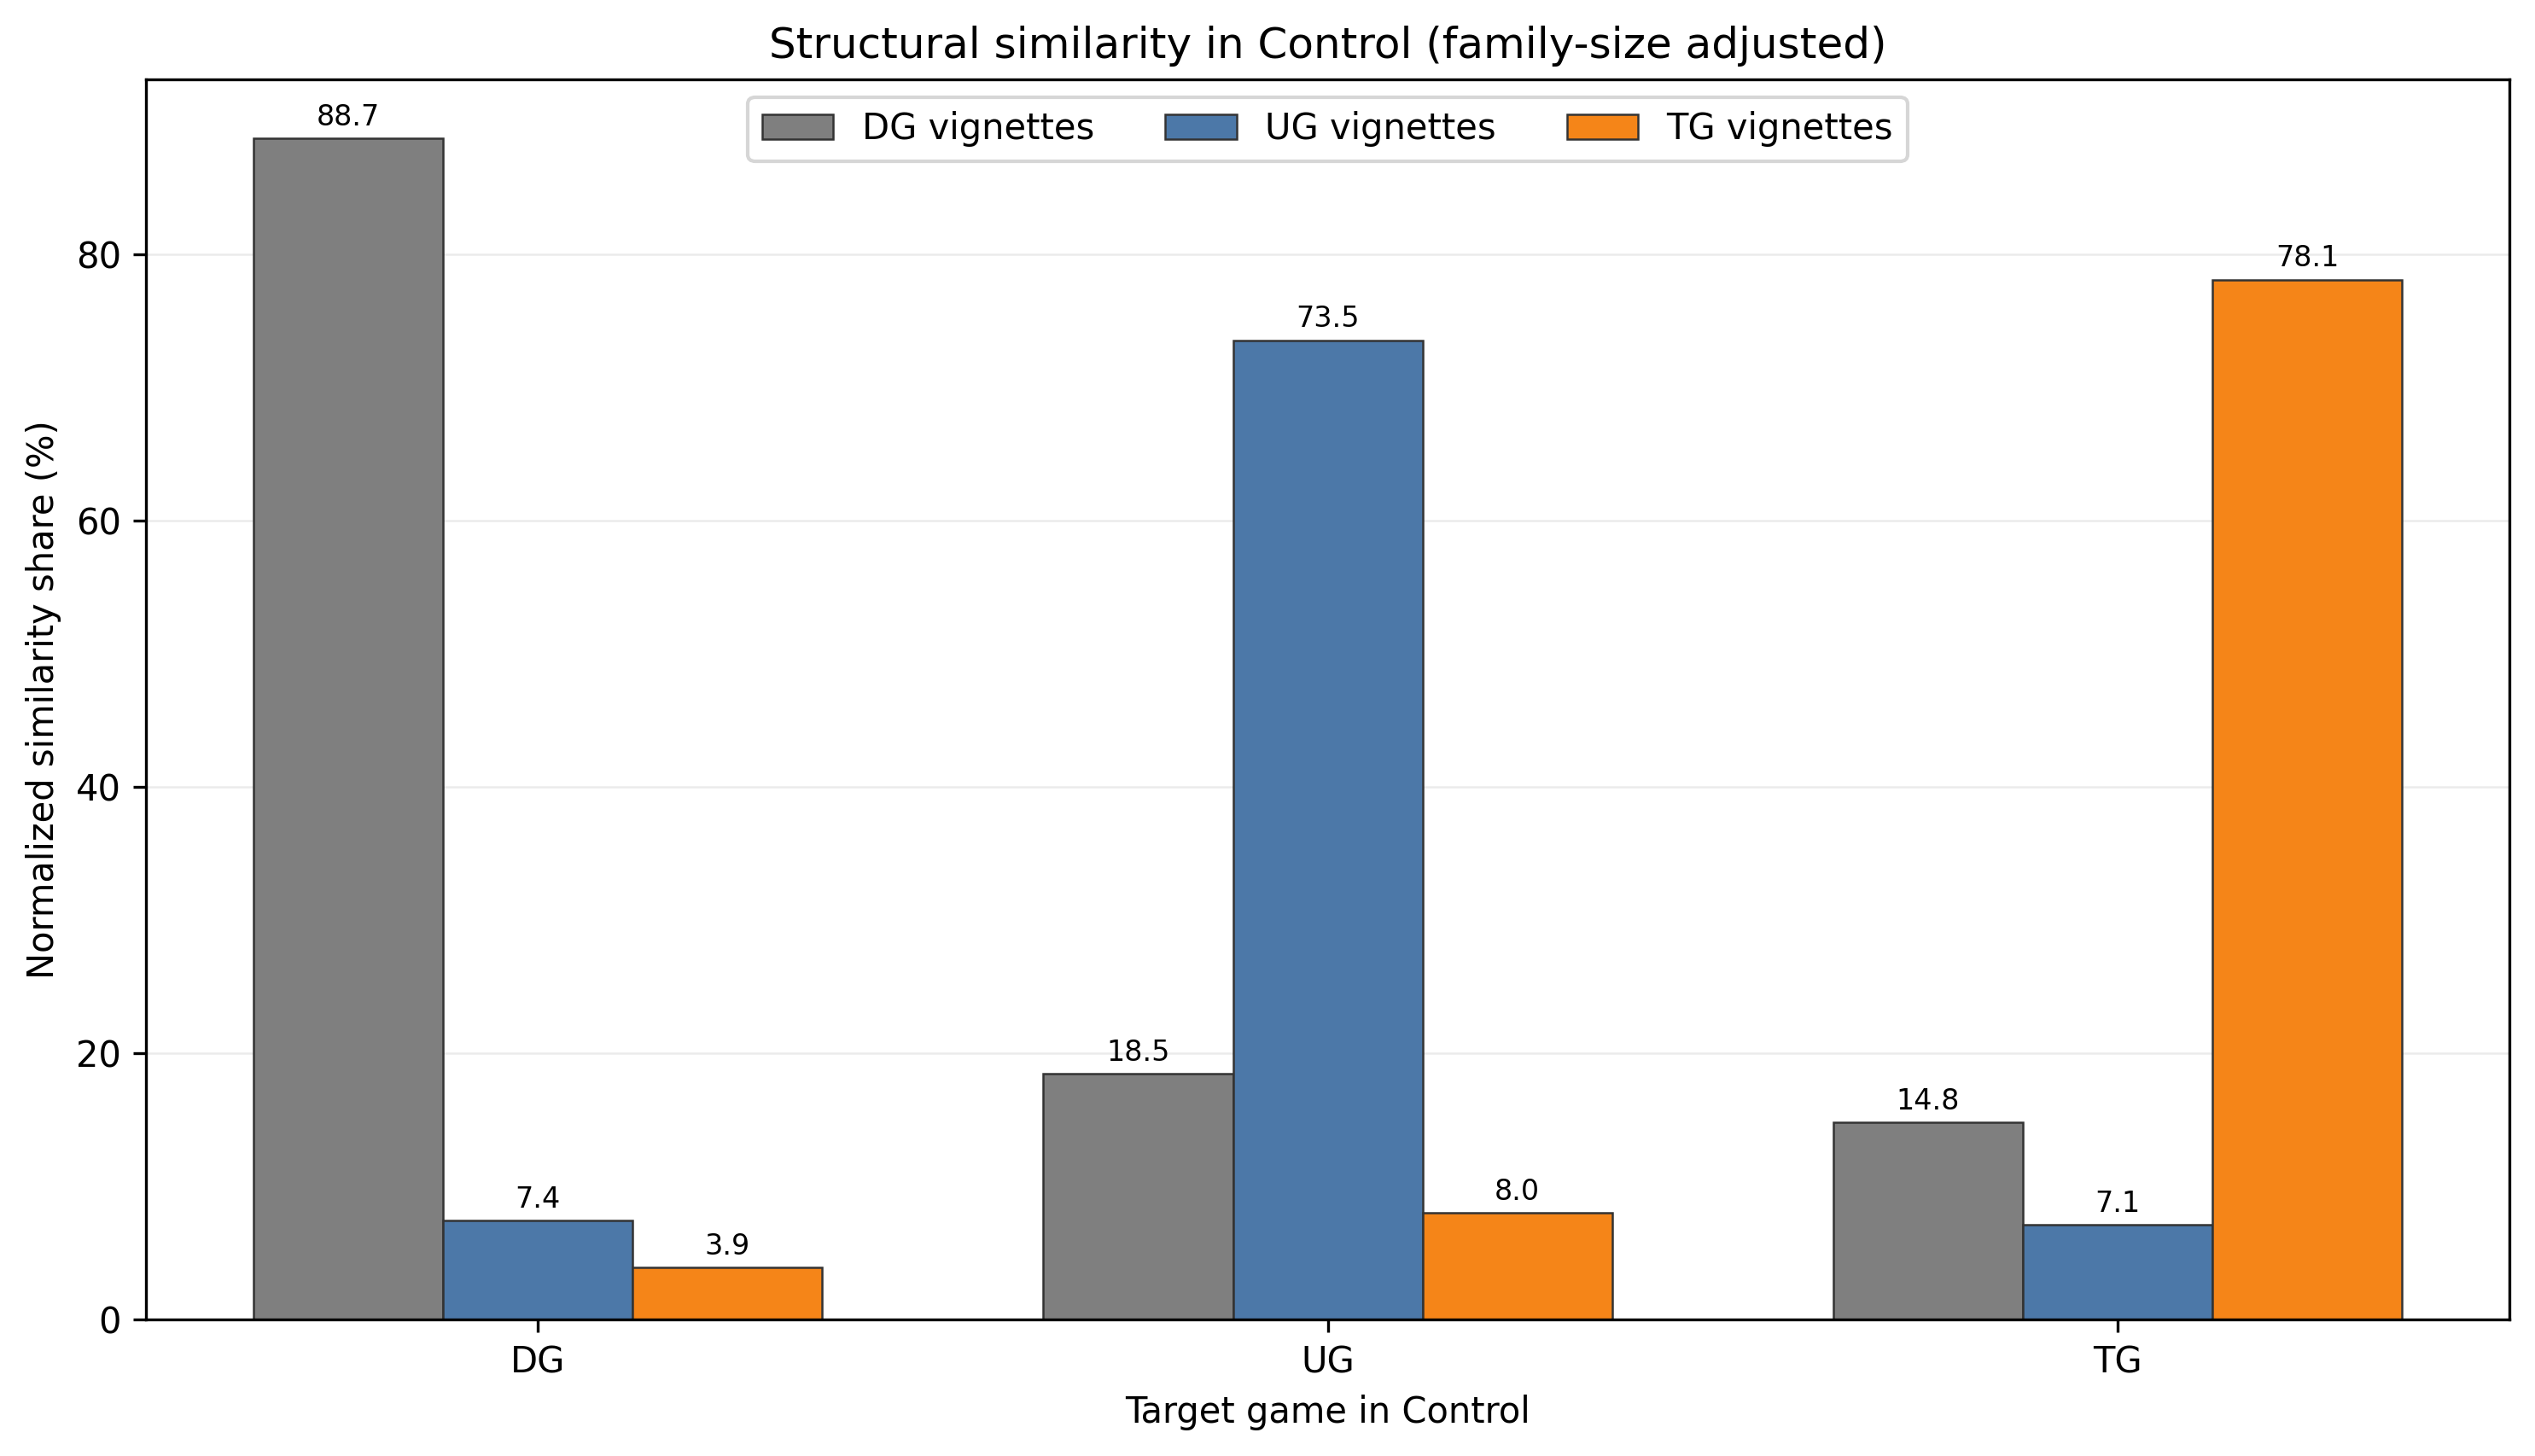
\includegraphics[width=0.98\textwidth]{relative_structural_control.png}
    \caption{Family-size-adjusted structural similarity shares for the three
    Control contexts. Within each target game, the three bars are the
    normalized family means and sum to 100 percent.}
    \label{fig:structural-control}
\end{figure}

\section{Stage 2: representations within game structure}

In the second stage, each context is rated in a new task containing only
vignettes constructed around the same game: 6 candidates for DG and 12 for UG
or TG. The 1,000-point budget is therefore reallocated separately within each
game-specific choice set. After rating, individual vignette points are summed
within representation class $k$ and expressed as a share,

\begin{equation}
    q_{ck}=\frac{1}{1{,}000}\sum_{v\in\mathcal{V}_{g,k}}\bar p_{cv},
    \qquad \sum_k q_{ck}=1.
\end{equation}

DG has three sender classes: Moral (M), Self-interest (S), and Cooperation
(C). UG and TG have six joint-action classes, formed by crossing the sender
class with receiver cooperation or defection: M-C, M-D, S-C, S-D, C-C, and
C-D. These classifications are used only after the similarity ratings have
been recorded.

\begin{figure}[H]
    \centering
    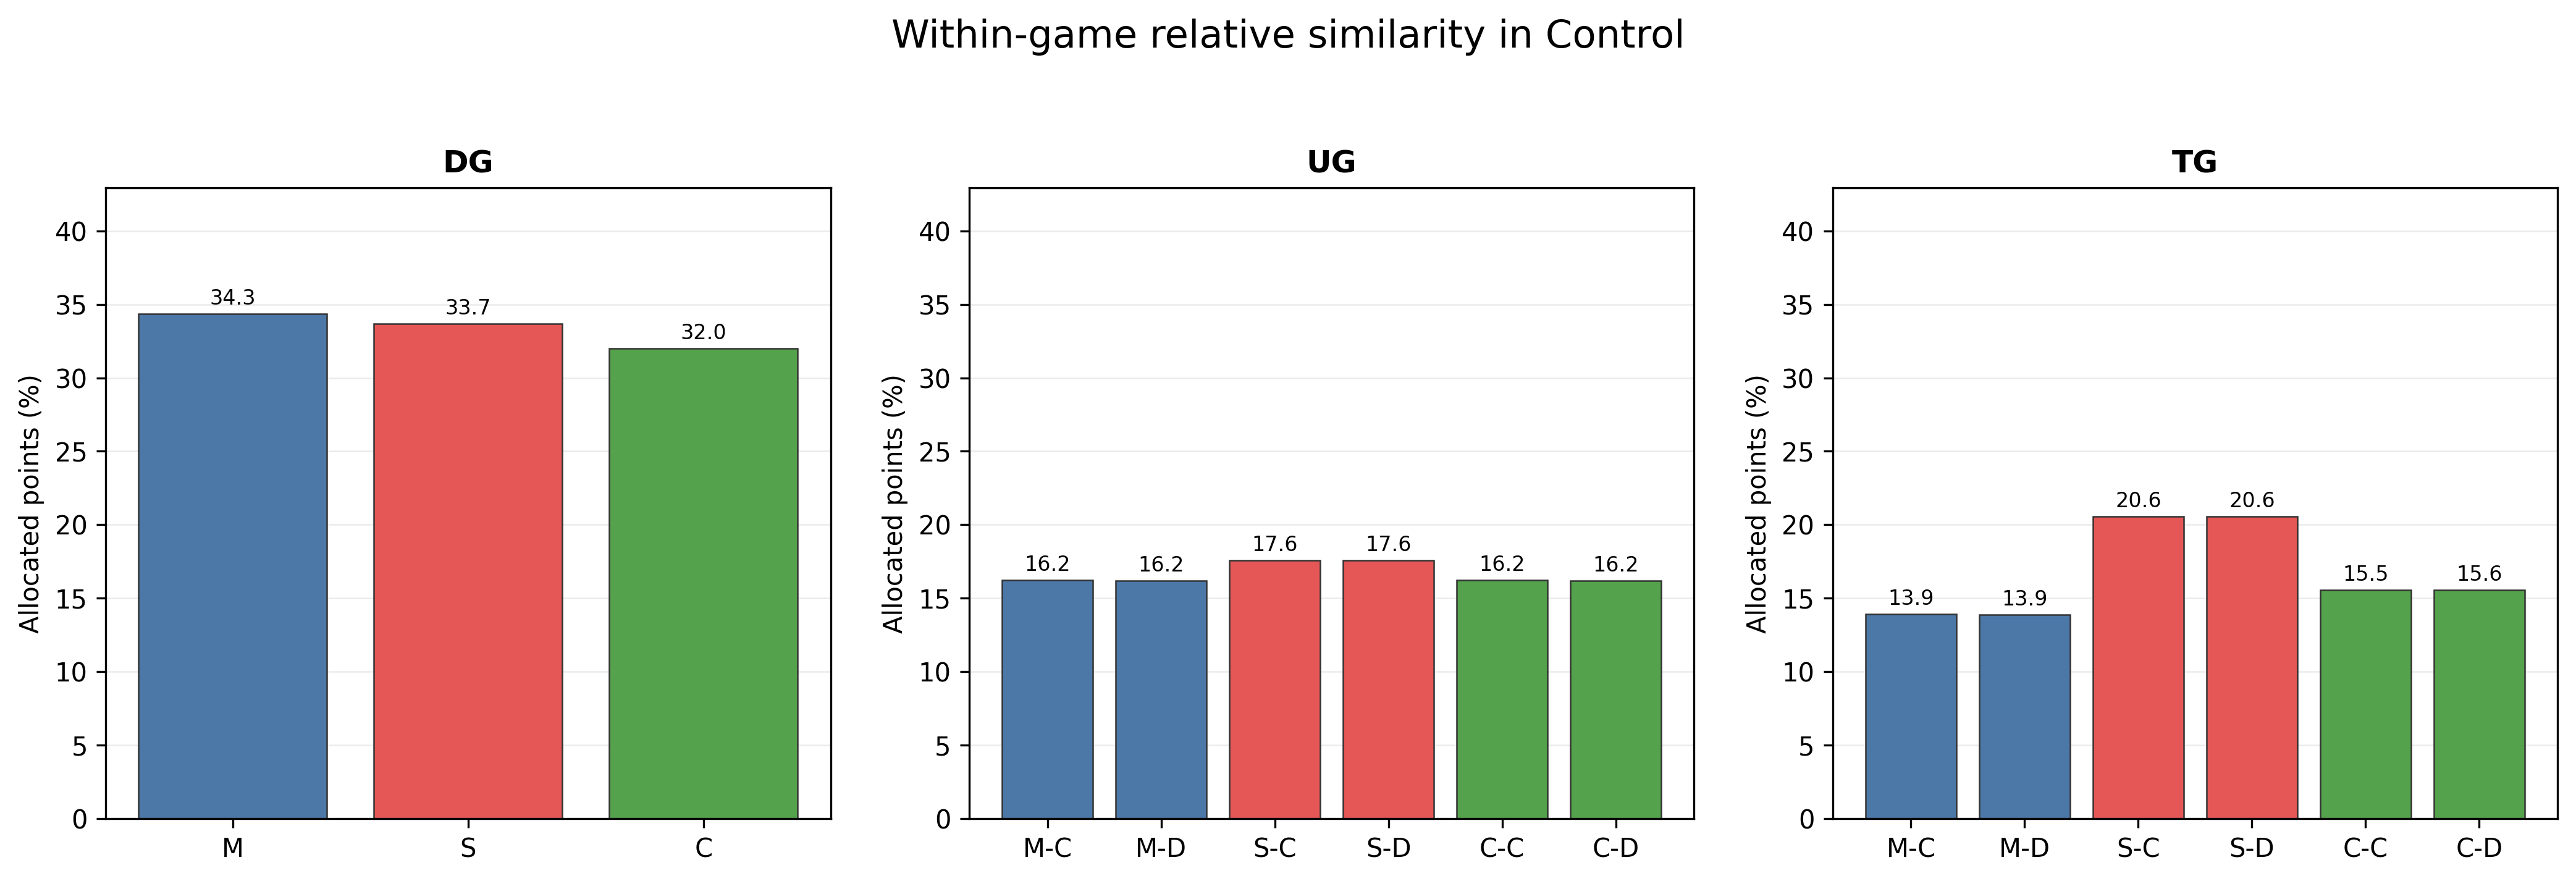
\includegraphics[width=0.98\textwidth]{relative_within_game_control.png}
    \caption{Within-game relative similarity in Control. Bars give each
    representation class's share of the 1,000 points and sum to 100 percent
    within each target game.}
    \label{fig:within-control}
\end{figure}

\begin{figure}[H]
    \centering
    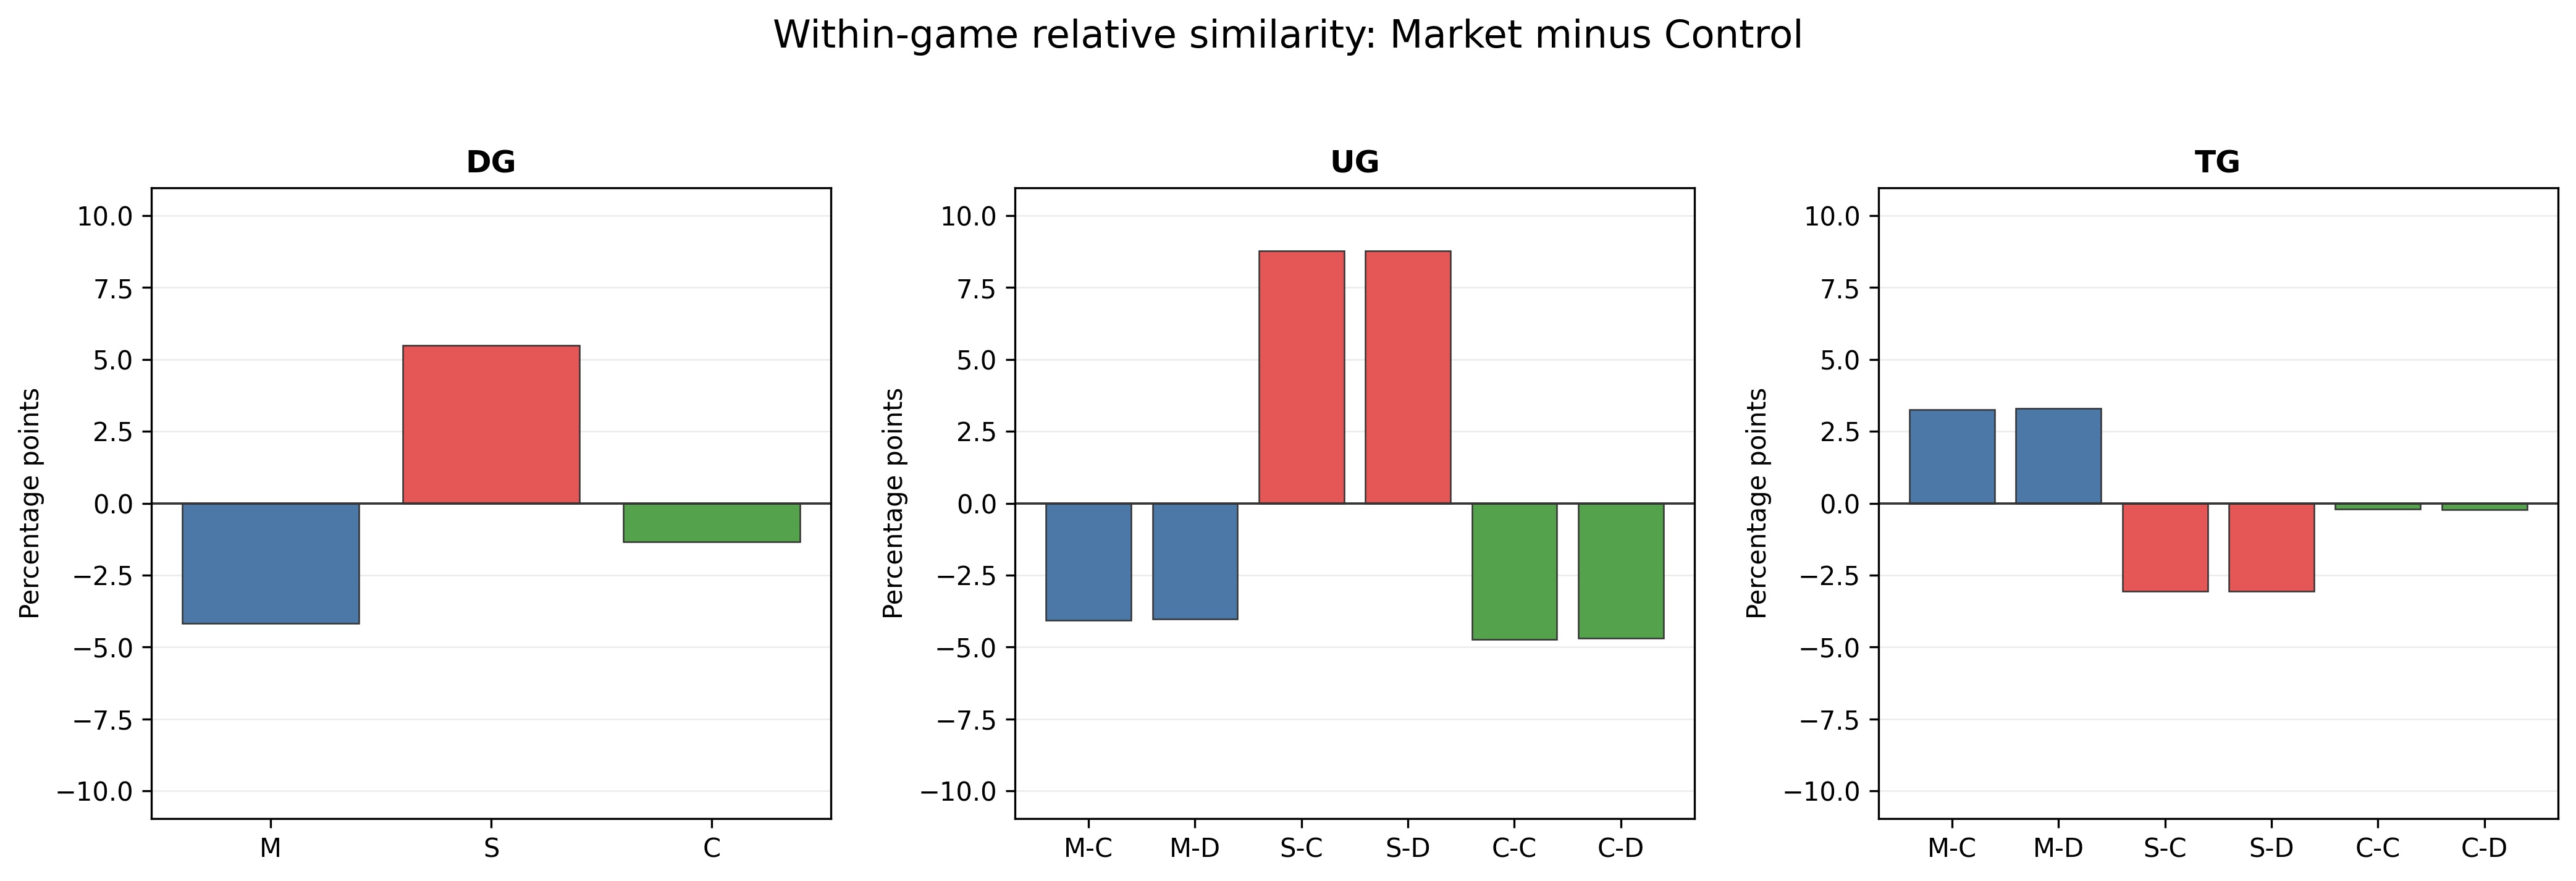
\includegraphics[width=0.98\textwidth]{relative_within_game_market_minus_control.png}
    \caption{Change in within-game representation shares: Market minus
    Control. Differences sum to zero within each target game.}
    \label{fig:within-market-control}
\end{figure}

\begin{figure}[H]
    \centering
    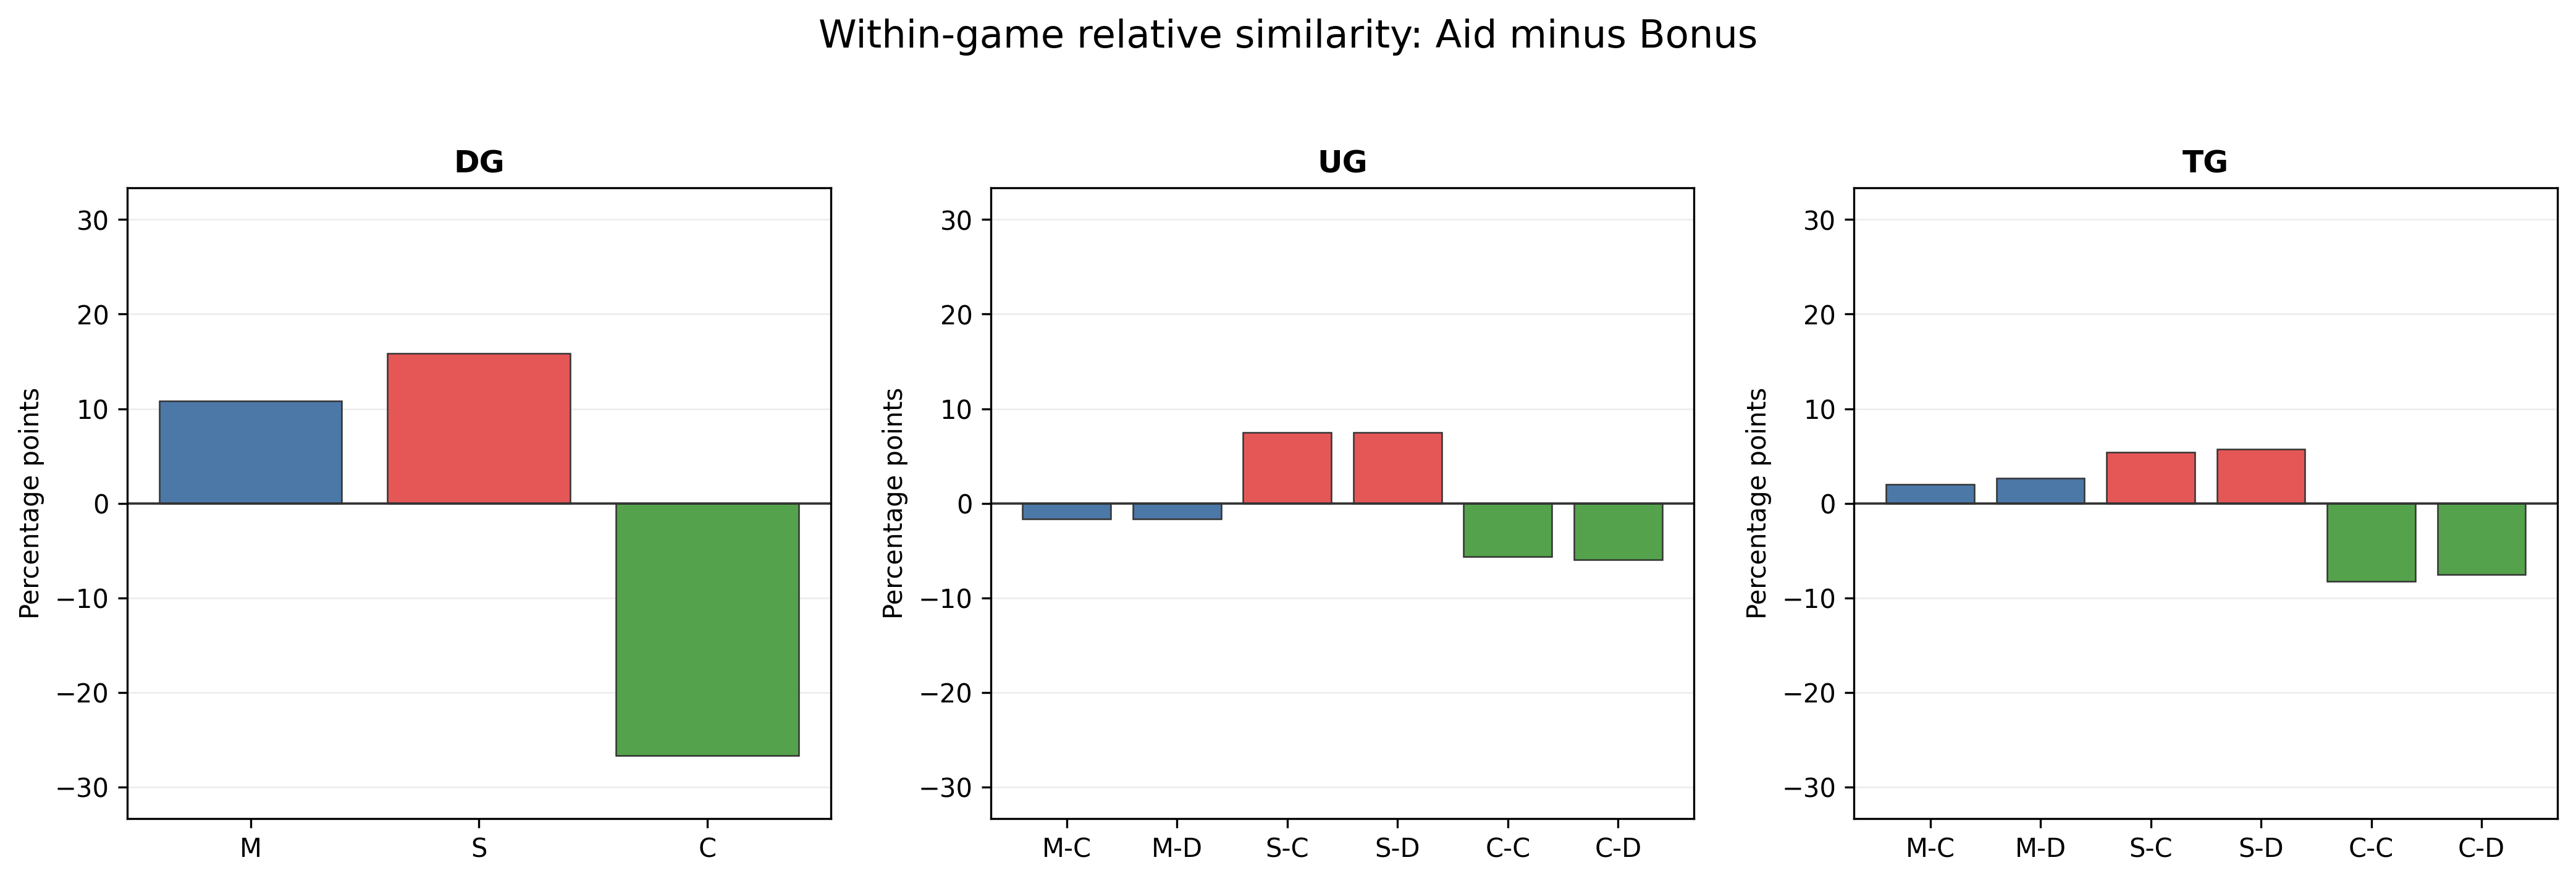
\includegraphics[width=0.98\textwidth]{relative_within_game_aid_minus_bonus.png}
    \caption{Change in within-game representation shares: Aid minus Bonus.
    Differences sum to zero within each target game.}
    \label{fig:within-aid-bonus}
\end{figure}

\end{document}
